\documentclass[a4paper, 11pt]{article}

\usepackage[spanish]{babel}
\usepackage[utf8]{inputenc}
\usepackage[T1]{fontenc}
\usepackage[vmargin=2cm,hmargin=2cm]{geometry}
\usepackage{graphicx}
\graphicspath{{img/}}
\usepackage{accents}
\usepackage{framed}

\title{\Huge \textbf{Práctica 1}}

\author{\textbf{Pablo Baeyens Fernández} \\ \textbf{Antonio Checa Molina} \\
\textbf{Iñaki Madinabeitia Cabrera} \\  \textbf{José Manuel Muñoz Fuentes} \\
 \textbf{Darío Sierra Martínez} \\ }

\date{Algorítmica}

\begin{document}

\maketitle
\tableofcontents

\newpage
\section{Ejercicio 1}
En el ejercicio 1 se nos pide hallar la eficiencia empírica de los algoritmos
presentados en la sesión. Para ello hemos modificado los códigos de los programas
para que tengan como salida el tamaño que se les pasó como argumento junto al tiempo
que han tardado en realizar la tarea del respectivo algoritmo.
Usando la biblioteca \textit{chrono} y la estructura que se menciona en la
sesión se consiguen medir los tiempos de los programas de forma precisa. \\

Una vez hecho esto, se elaboró un script de bash para automatizar la ejecución de
cada algoritmo con varios tamaños y recoger todas las salidas en un archivo para
luego poder usar esos datos. El script es el siguiente:


\begin{framed}

	\# !/bin/bash

	\# Uso: nombredelejecutable inicial salto final

	\# Ejemplo: fibonacci 10 5 80 ejecuta fibonacci 10, fibonacci 15, ..., fibonacci 80

	\# Salida: nombredelejecutable.dat
	\vspace{0.3cm}

	$>$ \$(basename \$1 .exe).dat

	for i in \$(seq \$2 \$3 \$4); do

	\hspace{0.4cm}./\$1 \$i $>>$ \$(basename \$1 .exe).dat

	done

\end{framed}

Las tablas generadas con este proceso se presentan a continuación, habiendo una tabla
para cada orden de eficiencia y una última tabla que reúne los tiempos de todos los
algoritmos de ordenación. \\

Todos los tiempos que se muestran en las tablas están en segundos, mientras que
\textit{Tamaño} menciona el tamaño total de la muestra con la que se obtuvo cada
tiempo de ejecución: en los algoritmos de ordenación hace referencia a la
capacidad del vector que se ordenaba, mientras que en Fibonacci o Hanói hace
referencia a las iteraciones totales del programa. \\

Debido al tamaño de las tablas (ya que cada una debía tener al menos 25 entradas),
cada tabla se muestra en una página. \\

Cabe destacar que la diferencia entre algoritmos de ordenación de un orden y de
otro resulta tan pronunciada que los algoritmos de orden $n \cdot \log (n)$ se
han ejecutado una segunda vez con un rango de valores en el que obtienen tiempos
de ejecución minúsculos, muchos órdenes de magnitud por debajo del obtenido por
los otros algoritmos de ordenación. En la tabla en la que se presentan se usan
tamaños mucho mayores, mientras que en la tabla comparativa de algoritmos de
ordenación toman estos mismos valores.

\subsection{Tabla del algoritmo de burbuja}
\begin{tabular}{|l|l|l|l|l|l|}
	\hline
	Tamaño & Antonio & Darío & Iñaki & José Manuel & Pablo \\
	\hline
	\hline
	2000 & 0,011413 & 0,0146897 & 0,0140894 & 0,00961352 & 0,00950047 \\
	\hline
	4000 & 0,0453449 & 0,0459751 & 0,0515536 & 0,0420678 & 0,0349755 \\
	\hline
	6000 & 0,101489 & 0,104199 & 0,113751 & 0,103764 & 0,0854343 \\
	\hline
	8000 & 0,181023 & 0,186132 & 0,202951 & 0,196277 & 0,157036 \\
	\hline
	10000 & 0,285049 & 0,292014 & 0,317834 & 0,319125 & 0,256134 \\
	\hline
	12000 & 0,412749 & 0,420102 & 0,467509 & 0,474853 & 0,377695 \\
	\hline
	14000 & 0,564313 & 0,575514 & 0,637843 & 0,657486 & 0,523751 \\
	\hline
	16000 & 0,736274 & 0,750603 & 0,831875 & 0,874744 & 0,6983 \\
	\hline
	18000 & 0,9231 & 0,957501 & 1,05149 & 1,12075 & 0,893985 \\
	\hline
	20000 & 1,14936 & 1,17477 & 1,2976 & 1,40219 & 1,11517 \\
	\hline
	22000 & 1,38726 & 1,47318 & 1,56672 & 1,7091 & 1,35403 \\
	\hline
	24000 & 1,64832 & 1,71407 & 1,85661 & 2,04022 & 1,62055 \\
	\hline
	26000 & 1,93603 & 2,30372 & 2,1866 & 2,41593 & 1,91995 \\
	\hline
	28000 & 2,24947 & 2,36352 & 2,52668 & 2,80527 & 2,24616 \\
	\hline
	30000 & 2,56848 & 2,68279 & 2,90867 & 3,23442 & 2,56361 \\
	\hline
	32000 & 2,92343 & 3,04424 & 3,32019 & 3,70037 & 2,92795 \\
	\hline
	34000 & 3,31074 & 3,46101 & 3,72809 & 4,20884 & 3,42199 \\
	\hline
	36000 & 3,71294 & 3,92597 & 4,19815 & 4,72597 & 3,73458 \\
	\hline
	38000 & 4,16954 & 4,7286 & 4,67249 & 5,28111 & 4,28892 \\
	\hline
	40000 & 4,74451 & 4,82232 & 5,15041 & 5,86181 & 4,73263 \\
	\hline
	42000 & 5,26566 & 5,59224 & 5,69877 & 6,46732 & 5,13279 \\
	\hline
	44000 & 5,87307 & 5,98763 & 6,25114 & 7,12322 & 5,6496 \\
	\hline
	46000 & 6,53502 & 6,63358 & 6,82935 & 7,80777 & 6,16936 \\
	\hline
	48000 & 7,32794 & 7,79745 & 7,43045 & 8,50997 & 6,76063 \\
	\hline
	50000 & 8,1269 & 7,95426 & 8,08572 & 9,2569 & 7,48556 \\
	\hline
\end{tabular}


\subsection{Tabla del algoritmo de selección}
\begin{tabular}{|l|l|l|l|l|l|}
	\hline
	Tamaño & Antonio & Darío & Iñaki & José Manuel & Pablo \\
	\hline
	\hline
	2000 & 0,00515467 & 0,0188928 & 0,0056981 & 0,00642196 & 0,0100637 \\
	\hline
	4000 & 0,019939 & 0,0519322 & 0,0229513 & 0,0256021 & 0,0289865 \\
	\hline
	6000 & 0,0433264 & 0,0570531 & 0,0484921 & 0,0570988 & 0,048992 \\
	\hline
	8000 & 0,0764116 & 0,0828212 & 0,085303 & 0,101468 & 0,0826678 \\
	\hline
	10000 & 0,121217 & 0,121786 & 0,133457 & 0,158756 & 0,126158 \\
	\hline
	12000 & 0,177811 & 0,175157 & 0,192178 & 0,22877 & 0,181783 \\
	\hline
	14000 & 0,244628 & 0,238585 & 0,260748 & 0,311101 & 0,249812 \\
	\hline
	16000 & 0,320919 & 0,310348 & 0,344565 & 0,416511 & 0,323524 \\
	\hline
	18000 & 0,410265 & 0,393202 & 0,436515 & 0,515545 & 0,409696 \\
	\hline
	20000 & 0,509134 & 0,484858 & 0,532265 & 0,636664 & 0,505402 \\
	\hline
	22000 & 0,61807 & 0,612123 & 0,647896 & 0,770943 & 0,611046 \\
	\hline
	24000 & 0,739096 & 0,697154 & 0,765415 & 0,92343 & 0,727033 \\
	\hline
	26000 & 0,872412 & 0,817823 & 0,902801 & 1,07721 & 0,853734 \\
	\hline
	28000 & 1,01093 & 0,949272 & 1,04346 & 1,25703 & 0,990795 \\
	\hline
	30000 & 1,16345 & 1,08959 & 1,20025 & 1,43408 & 1,13651 \\
	\hline
	32000 & 1,33592 & 1,33227 & 1,36391 & 1,63213 & 1,30253 \\
	\hline
	34000 & 1,50895 & 1,62408 & 1,5385 & 1,84905 & 1,46012 \\
	\hline
	36000 & 1,70088 & 1,71456 & 1,72302 & 2,07075 & 1,63606 \\
	\hline
	38000 & 1,91222 & 1,89498 & 1,91741 & 2,30688 & 1,82284 \\
	\hline
	40000 & 2,12327 & 2,27765 & 2,12458 & 2,56224 & 2,0183 \\
	\hline
	42000 & 2,35229 & 2,29655 & 2,34051 & 2,81587 & 2,22564 \\
	\hline
	44000 & 2,60759 & 2,42883 & 2,56741 & 3,09183 & 2,44306 \\
	\hline
	46000 & 2,8435 & 2,9669 & 2,80465 & 3,37761 & 2,67054 \\
	\hline
	48000 & 3,11111 & 3,185 & 3,05395 & 3,66923 & 2,90848 \\
	\hline
	50000 & 3,40647 & 3,47501 & 3,3125 & 3,98744 & 3,15386 \\
	\hline
\end{tabular}


\subsection{Tabla del algoritmo de inserción}
\begin{tabular}{|l|l|l|l|l|l|}
	\hline
	Tamaño & Antonio & Darío & Iñaki & José Manuel & Pablo \\
	\hline
	\hline
	2000 & 0,0044917 & 0,00745713 & 0,00500529 & 0,00545271 & 0,0136858 \\
	\hline
	4000 & 0,0186884 & 0,0182933 & 0,0211343 & 0,0212218 & 0,0240584 \\
	\hline
	6000 & 0,0377812 & 0,0394224 & 0,0423133 & 0,0478191 & 0,0388833 \\
	\hline
	8000 & 0,0669812 & 0,0683471 & 0,0749079 & 0,0855453 & 0,07279 \\
	\hline
	10000 & 0,107932 & 0,107475 & 0,119386 & 0,139938 & 0,106441 \\
	\hline
	12000 & 0,154884 & 0,153773 & 0,171897 & 0,191814 & 0,153352 \\
	\hline
	14000 & 0,213453 & 0,209259 & 0,230161 & 0,259945 & 0,207844 \\
	\hline
	16000 & 0,280269 & 0,271604 & 0,306819 & 0,348722 & 0,272146 \\
	\hline
	18000 & 0,368311 & 0,345483 & 0,394836 & 0,43881 & 0,344915 \\
	\hline
	20000 & 0,443013 & 0,426531 & 0,471464 & 0,535028 & 0,423007 \\
	\hline
	22000 & 0,541246 & 0,644623 & 0,575623 & 0,642579 & 0,512299 \\
	\hline
	24000 & 0,649446 & 0,614673 & 0,669068 & 0,768137 & 0,615278 \\
	\hline
	26000 & 0,760331 & 0,903855 & 0,816444 & 0,903978 & 0,711269 \\
	\hline
	28000 & 0,882182 & 0,950041 & 0,915119 & 1,05197 & 0,828786 \\
	\hline
	30000 & 1,03487 & 1,06675 & 1,05814 & 1,20102 & 0,947152 \\
	\hline
	32000 & 1,18717 & 1,11084 & 1,19949 & 1,37548 & 1,07939 \\
	\hline
	34000 & 1,33726 & 1,76733 & 1,35952 & 1,53781 & 1,21549 \\
	\hline
	36000 & 1,51744 & 1,5771 & 1,51431 & 1,7434 & 1,3987 \\
	\hline
	38000 & 1,70203 & 1,88235 & 1,68403 & 1,92846 & 1,51493 \\
	\hline
	40000 & 1,87561 & 1,94893 & 1,88228 & 2,15878 & 1,68276 \\
	\hline
	42000 & 2,08887 & 2,29417 & 2,09879 & 2,34337 & 1,84894 \\
	\hline
	44000 & 2,30682 & 2,12463 & 2,26926 & 2,58382 & 2,02091 \\
	\hline
	46000 & 2,54603 & 2,73282 & 2,46238 & 2,82213 & 2,22809 \\
	\hline
	48000 & 2,79809 & 2,59309 & 2,66613 & 3,07817 & 2,41128 \\
	\hline
	50000 & 3,02904 & 3,52064 & 2,92835 & 3,32697 & 2,62017 \\
	\hline
\end{tabular}


\subsection{Tabla de los algoritmos cuadráticos}
<<<<<<< HEAD

\begin{tabular}{|l|l|l|l|}
	\hline
	Tamaño &Tiempo de Burbuja &Tiempo de  Inserción &Tiempo de  Selección \\
	\hline
	\hline
	2000 & 0,0141 & 0,005 & 0,0057 \\
	\hline
	4000 & 0,0516 & 0,0211 & 0,023 \\
	\hline
	6000 & 0,1138 & 0,0423 & 0,0485 \\
	\hline
	8000 & 0,203 & 0,0749 & 0,0853 \\
	\hline
	10000 & 0,3178 & 0,1194 & 0,1335 \\
	\hline
	12000 & 0,4675 & 0,1719 & 0,1922 \\
	\hline
	14000 & 0,6378 & 0,2302 & 0,2608 \\
	\hline
	16000 & 0,8319 & 0,3068 & 0,3446 \\
	\hline
	18000 & 1,0515 & 0,3948 & 0,4365 \\
	\hline
	20000 & 1,2976 & 0,4715 & 0,5323 \\
	\hline
	22000 & 1,5667 & 0,5756 & 0,6479 \\
	\hline
	24000 & 1,8566 & 0,6691 & 0,7654 \\
	\hline
	26000 & 2,1866 & 0,8164 & 0,9028 \\
	\hline
	28000 & 2,5267 & 0,9151 & 1,0435 \\
	\hline
	30000 & 2,9087 & 1,0581 & 1,2003 \\
	\hline
	32000 & 3,3202 & 1,1995 & 1,3639 \\
	\hline
	34000 & 3,7281 & 1,3595 & 1,5385 \\
	\hline
	36000 & 4,1982 & 1,5143 & 1,723 \\
	\hline
	38000 & 4,6725 & 1,684 & 1,9174 \\
	\hline
	40000 & 5,1504 & 1,8823 & 2,1246 \\
	\hline
	42000 & 5,6988 & 2,0988 & 2,3405 \\
	\hline
	44000 & 6,2511 & 2,2693 & 2,5674 \\
	\hline
	46000 & 6,8294 & 2,4624 & 2,8047 \\
	\hline
	48000 & 7,4305 & 2,6661 & 3,054 \\
	\hline
	50000 & 8,0857 & 2,9284 & 3,3125 \\
	\hline
\end{tabular}

\subsection{Tabla de los algoritmos $n\cdot \log(n)$ }
=======

Incluimos una tabla comparando los datos de una sóla persona para los algoritmos
de orden cuadrático:

\begin{tabular}{|l|l|l|l|}
	\hline
	Tamaño &Tiempo de Burbuja &Tiempo de  Inserción &Tiempo de  Selección \\
	\hline
	\hline
	2000 & 0,0141 & 0,005 & 0,0057 \\
	\hline
	4000 & 0,0516 & 0,0211 & 0,023 \\
	\hline
	6000 & 0,1138 & 0,0423 & 0,0485 \\
	\hline
	8000 & 0,203 & 0,0749 & 0,0853 \\
	\hline
	10000 & 0,3178 & 0,1194 & 0,1335 \\
	\hline
	12000 & 0,4675 & 0,1719 & 0,1922 \\
	\hline
	14000 & 0,6378 & 0,2302 & 0,2608 \\
	\hline
	16000 & 0,8319 & 0,3068 & 0,3446 \\
	\hline
	18000 & 1,0515 & 0,3948 & 0,4365 \\
	\hline
	20000 & 1,2976 & 0,4715 & 0,5323 \\
	\hline
	22000 & 1,5667 & 0,5756 & 0,6479 \\
	\hline
	24000 & 1,8566 & 0,6691 & 0,7654 \\
	\hline
	26000 & 2,1866 & 0,8164 & 0,9028 \\
	\hline
	28000 & 2,5267 & 0,9151 & 1,0435 \\
	\hline
	30000 & 2,9087 & 1,0581 & 1,2003 \\
	\hline
	32000 & 3,3202 & 1,1995 & 1,3639 \\
	\hline
	34000 & 3,7281 & 1,3595 & 1,5385 \\
	\hline
	36000 & 4,1982 & 1,5143 & 1,723 \\
	\hline
	38000 & 4,6725 & 1,684 & 1,9174 \\
	\hline
	40000 & 5,1504 & 1,8823 & 2,1246 \\
	\hline
	42000 & 5,6988 & 2,0988 & 2,3405 \\
	\hline
	44000 & 6,2511 & 2,2693 & 2,5674 \\
	\hline
	46000 & 6,8294 & 2,4624 & 2,8047 \\
	\hline
	48000 & 7,4305 & 2,6661 & 3,054 \\
	\hline
	50000 & 8,0857 & 2,9284 & 3,3125 \\
	\hline
\end{tabular}

\subsection{Tabla del algoritmo Heapsort}
\begin{tabular}{|l|l|l|l|l|l|}
	\hline
	Tamaño & Antonio & Darío & Iñaki & José Manuel & Pablo \\
	\hline
	\hline
	1000000 & 0,22421 & 0,29581 & 0,252793 & 0,305145 & 0,298779 \\
	\hline
	2000000 & 0,500762 & 0,488327 & 0,557837 & 0,687773 & 0,516744 \\
	\hline
	3000000 & 0,833796 & 0,862668 & 0,923097 & 1,13871 & 0,816685 \\
	\hline
	4000000 & 1,17323 & 1,30803 & 1,26719 & 1,56775 & 1,15558 \\
	\hline
	5000000 & 1,54404 & 1,77557 & 1,66226 & 2,03485 & 1,52638 \\
	\hline
	6000000 & 1,9243 & 1,99408 & 2,06275 & 2,53414 & 1,85543 \\
	\hline
	7000000 & 2,35331 & 2,48359 & 2,46109 & 3,03014 & 2,24277 \\
	\hline
	8000000 & 2,76399 & 2,86937 & 2,89135 & 3,53461 & 2,61264 \\
	\hline
	9000000 & 3,20945 & 3,38923 & 3,30651 & 4,05931 & 2,98857 \\
	\hline
	10000000 & 3,62159 & 3,97747 & 3,69426 & 4,57383 & 3,34685 \\
	\hline
	11000000 & 4,09924 & 4,16954 & 4,14343 & 5,11395 & 3,77043 \\
	\hline
	12000000 & 4,63249 & 4,54798 & 4,6038 & 5,64885 & 4,12332 \\
	\hline
	13000000 & 5,0709 & 5,08649 & 5,06756 & 6,19867 & 4,54708 \\
	\hline
	14000000 & 5,55749 & 5,5935 & 5,51359 & 6,73735 & 4,94788 \\
	\hline
	15000000 & 6,13142 & 5,77158 & 5,96415 & 7,31606 & 5,38968 \\
	\hline
	16000000 & 6,57542 & 6,79831 & 6,40422 & 7,86827 & 5,78389 \\
	\hline
	17000000 & 7,11513 & 6,95513 & 6,93151 & 8,42371 & 6,22592 \\
	\hline
	18000000 & 7,60767 & 7,84526 & 7,39067 & 9,00969 & 6,58787 \\
	\hline
	19000000 & 8,18748 & 7,61565 & 7,85371 & 9,5756 & 7,03859 \\
	\hline
	20000000 & 8,6704 & 8,15118 & 8,35113 & 10,1822 & 7,4932 \\
	\hline
	21000000 & 9,14739 & 8,49386 & 8,85375 & 10,7763 & 7,98279 \\
	\hline
	22000000 & 9,68533 & 8,7519 & 9,26481 & 11,3518 & 8,33516 \\
	\hline
	23000000 & 10,1561 & 12,3292 & 9,70679 & 11,9304 & 8,76102 \\
	\hline
	24000000 & 10,6587 & 11,7971 & 10,2619 & 12,4831 & 9,21482 \\
	\hline
	25000000 & 11,2477 & 11,9356 & 10,7142 & 13,1053 & 9,69064 \\
	\hline
\end{tabular}

\subsection{Tabla del algoritmo Mergesort}
\begin{tabular}{|l|l|l|l|l|l|}
	\hline
	Tamaño & Antonio & Darío & Iñaki & José Manuel & Pablo \\
	\hline
	\hline
	2000 & 0,000357711 & 0,41989 & 0,245436 & 0,301188 & 0,260094 \\
	\hline
	4000 & 0,000733633 & 0,944787 & 0,508929 & 0,624731 & 0,477345 \\
	\hline
	6000 & 0,00129252 & 1,60546 & 0,883956 & 1,0693 & 0,817615 \\
	\hline
	8000 & 0,00141135 & 1,76623 & 1,06884 & 1,30794 & 0,991948 \\
	\hline
	10000 & 0,00173272 & 2,59677 & 1,42201 & 1,74213 & 1,32955 \\
	\hline
	12000 & 0,00250515 & 3,23115 & 1,80438 & 2,24784 & 1,70433 \\
	\hline
	14000 & 0,00237975 & 3,125 & 1,88077 & 2,33259 & 1,74689 \\
	\hline
	16000 & 0,00353891 & 4,02999 & 2,21405 & 2,75695 & 2,06821 \\
	\hline
	18000 & 0,00317823 & 4,73714 & 2,56327 & 3,17912 & 2,40275 \\
	\hline
	20000 & 0,00372753 & 5,95524 & 2,94302 & 3,60459 & 2,75836 \\
	\hline
	22000 & 0,00416415 & 6,1202 & 3,32014 & 4,10528 & 3,20704 \\
	\hline
	24000 & 0,00475486 & 6,88797 & 3,73637 & 4,58481 & 3,46971 \\
	\hline
	26000 & 0,00422964 & 6,84617 & 4,03523 & 5,08856 & 3,76172 \\
	\hline
	28000 & 0,00478424 & 6,15036 & 3,89364 & 4,83557 & 3,61966 \\
	\hline
	30000 & 0,0050692 & 7,34219 & 4,24867 & 5,24825 & 3,94948 \\
	\hline
	32000 & 0,00548591 & 8,05125 & 4,57914 & 5,70737 & 4,26975 \\
	\hline
	34000 & 0,00589953 & 7,76039 & 4,95366 & 6,13015 & 4,61115 \\
	\hline
	36000 & 0,00653509 & 7,92355 & 5,30502 & 6,56022 & 4,93584 \\
	\hline
	38000 & 0,00691745 & 8,92073 & 5,67961 & 7,13455 & 5,27359 \\
	\hline
	40000 & 0,00767938 & 10,3971 & 6,07057 & 7,49875 & 5,64695 \\
	\hline
	42000 & 0,00798031 & 10,9268 & 6,45905 & 7,96927 & 6,0763 \\
	\hline
	44000 & 0,00866207 & 11,7692 & 6,86264 & 8,45273 & 6,3987 \\
	\hline
	46000 & 0,00916131 & 11,9725 & 7,27508 & 9,01187 & 6,76389 \\
	\hline
	48000 & 0,00982215 & 12,1088 & 7,76361 & 9,49399 & 7,15444 \\
	\hline
	50000 & 0,0106109 & 12,8678 & 8,11788 & 10,0094 & 7,57097 \\
	\hline
\end{tabular}

\subsection{Tabla del algoritmo Quicksort}
\begin{tabular}{|l|l|l|l|l|l|}
	\hline
	Tamaño & Antonio & Darío & Iñaki & José Manuel & Pablo \\
	\hline
	\hline
	1000000 & 0,140354 & 0,184352 & 0,158862 & 0,201315 & 0,151376 \\
	\hline
	2000000 & 0,290671 & 0,30058 & 0,333955 & 0,417716 & 0,315613 \\
	\hline
	3000000 & 0,451042 & 0,661469 & 0,51239 & 0,647102 & 0,493536 \\
	\hline
	4000000 & 0,609228 & 0,782993 & 0,689444 & 0,891546 & 0,677623 \\
	\hline
	5000000 & 0,768809 & 0,958429 & 0,87572 & 1,10639 & 0,834242 \\
	\hline
	6000000 & 0,939232 & 1,24997 & 1,06316 & 1,35262 & 1,02652 \\
	\hline
	7000000 & 1,09785 & 1,55516 & 1,25421 & 1,58457 & 1,19163 \\
	\hline
	8000000 & 1,26473 & 1,56534 & 1,44825 & 1,84108 & 1,37806 \\
	\hline
	9000000 & 1,43536 & 2,0214 & 1,63635 & 2,06708 & 1,57758 \\
	\hline
	10000000 & 1,62045 & 1,93912 & 1,80254 & 2,32434 & 1,72557 \\
	\hline
	11000000 & 1,79408 & 2,53682 & 2,01344 & 2,56235 & 1,95905 \\
	\hline
	12000000 & 1,95441 & 2,36726 & 2,21136 & 2,79477 & 2,10258 \\
	\hline
	13000000 & 2,12925 & 2,98066 & 2,39937 & 3,06728 & 2,30709 \\
	\hline
	14000000 & 2,30318 & 3,0189 & 2,58933 & 3,31356 & 2,50474 \\
	\hline
	15000000 & 2,45234 & 4,09368 & 2,78644 & 3,58529 & 2,68512 \\
	\hline
	16000000 & 2,62369 & 4,13583 & 2,98485 & 3,78366 & 2,83059 \\
	\hline
	17000000 & 2,81701 & 4,44071 & 3,17474 & 4,04963 & 3,04674 \\
	\hline
	18000000 & 3,02744 & 5,05181 & 3,35808 & 4,28425 & 3,22857 \\
	\hline
	19000000 & 3,26244 & 5,36954 & 3,56303 & 4,53229 & 3,41292 \\
	\hline
	20000000 & 3,44172 & 5,0034 & 3,80315 & 4,80884 & 3,59846 \\
	\hline
	21000000 & 3,69781 & 5,38552 & 3,95077 & 5,0512 & 3,77894 \\
	\hline
	22000000 & 3,94126 & 4,58768 & 4,17141 & 5,31982 & 3,93762 \\
	\hline
	23000000 & 4,20059 & 5,19099 & 4,37102 & 5,52691 & 4,11956 \\
	\hline
	24000000 & 4,36635 & 5,74367 & 4,55899 & 5,80511 & 4,35852 \\
	\hline
	25000000 & 4,59738 & 6,59753 & 4,77483 & 6,07513 & 4,53331 \\
	\hline
\end{tabular}


\subsection{Tabla de los algoritmos $n\cdot \log(n)$}

Incluimos una tabla comparando los datos de una sóla persona para los algoritmos
de orden $n\cdot \log(n)$:
>>>>>>> master

\begin{tabular}{|l|l|l|l|}
	\hline
	Tamaño & Tiempo de Heapsort & Tiempo de Mergesort & Tiempo de Quicksort \\
	\hline
	\hline
	1000000	&0,158862&	0,25279&	0,245436\\
	\hline
	2000000	&0,333955&	0,55784	&0,508929\\
	\hline
	3000000	&0,512390&	0,92310	&0,883956\\
	\hline
	4000000	&0,689444&	1,26719	&1,068840\\
	\hline
	5000000	&0,875720&	1,66226	&1,422010\\
	\hline
	6000000	&1,063160&	2,06275	&1,804380\\
	\hline
	7000000	&1,254210&	2,46109	&1,880770\\
	\hline
	8000000	&1,448250&	2,89135	&2,214050\\
	\hline
	9000000	&1,636350&	3,30651	&2,563270\\
	\hline
	10000000	&1,802540&	3,69426	&2,943020\\
	\hline
	11000000	&2,013440&	4,14343	&3,320140\\
	\hline
	12000000	&2,211360&	4,60380	&3,736370\\
	\hline
	13000000	&2,399370&	5,06756	&4,035230\\
	\hline
	14000000	&2,589330&	5,51359	&3,893640\\
	\hline
	15000000	&2,786440&	5,96415	&4,248670\\
	\hline
	16000000	&2,984850&	6,40422	&4,579140\\
	\hline
	17000000	&3,174740&	6,93151	&4,953660\\
	\hline
	18000000	&3,358080&	7,39067	&5,305020\\
	\hline
	19000000	&3,563030&	7,85371	&5,679610\\
	\hline
	20000000	&3,803150&	8,35113	&6,070570\\
	\hline
	21000000	&3,950770&	8,85375	&6,459050\\
	\hline
	22000000	&4,171410&	9,26481	&6,862640\\
	\hline
	23000000	&4,371020&	9,70679	&7,275080\\
	\hline
	24000000	&4,558990&	10,26190	&7,763610\\
	\hline
	25000000	&4,774830&	10,71420	&8,117880\\
	\hline
\end{tabular}

\subsection{Tabla del algoritmo cúbico (Floyd)}


\begin{tabular}{|l|l|}
	\hline
	Tamaño & Tiempo de Floyd \\
	\hline
	\hline
	30	&0,000280424\\
	\hline
	60	&0,001601650\\
	\hline
	90	&0,005779860\\
	\hline
	120	&0,011250300\\
	\hline
	150	&0,021107200\\
	\hline
	180	&0,035468500\\
	\hline
	210	&0,055724200\\
	\hline
	240	&0,082467900\\
	\hline
	270	&0,119058000\\
	\hline
	300	&0,160319000\\
	\hline
	330	&0,213182000\\
	\hline
	360	&0,281825000\\
	\hline
	390	&0,358154000\\
	\hline
	420	&0,437591000\\
	\hline
	450	&0,543534000\\
	\hline
	480	&0,652500000\\
	\hline
	510	&0,790683000\\
	\hline
	540	&0,929593000\\
	\hline
	570	&1,097870000\\
	\hline
	600	&1,279820000\\
	\hline
	630	&1,479150000\\
	\hline
	660	&1,703250000\\
	\hline
	690	&1,941560000\\
	\hline
	720	&2,199710000\\
	\hline
	750	&2,485840000\\
	\hline
\end{tabular}

\subsection{Tabla del algoritmo de Fibonacci $(O(\frac{1+\sqrt{5}}{2})^n)$}


\begin{tabular}{|l|l|}
	\hline
	Tamaño & Tiempo de Fibonacci \\
	\hline
	\hline
1&1.79e-07 \\
\hline
2&1.88e-07\\
\hline
3&2.05e-07\\
\hline
4&2.89e-07\\
\hline
5&2.61e-07\\
\hline
6&2.87e-07\\
\hline
7&4.65e-07\\
\hline
8&7.53e-07\\
\hline
9&1.131e-06\\
\hline
10&1.365e-06\\
\hline
11&1.796e-06\\
\hline
12&1.671e-06\\
\hline
13&3.612e-06\\
\hline
14&7.294e-06\\
\hline
15&7.834e-06\\
\hline
16&1.2102e-05\\
\hline
17&1.7977e-05\\
\hline
18&2.9478e-05\\
\hline
19&5.3614e-05\\
\hline
20&7.2343e-05\\
\hline
21&0.000132759\\
\hline
22&0.000189094\\
\hline
23&0.000315282\\
\hline
24&0.000499445\\
\hline
25&0.000675111\\
\hline

\end{tabular}

\subsection{Tabla del algoritmo de Hanoi ($O(2^n)$)}
\begin{tabular}{|l|l|}
	\hline
	Tamaño & Tiempo de Hanoi \\
	\hline
	\hline
1&1.85e-07\\
\hline
2&2.52e-07\\
\hline
3&3.63e-07\\
\hline
4&5.65e-07\\
\hline
5&5.96e-07\\
\hline
6&1.206e-06\\
\hline
7&1.909e-06\\
\hline
8&3.047e-06\\
\hline
9&5.639e-06\\
\hline
10&1.1064e-05\\
\hline
11&2.1002e-05\\
\hline
12&3.7705e-05\\
\hline
13&7.8102e-05\\
\hline
14&0.000165379\\
\hline
15&0.000334135\\
\hline
16&0.000589484\\
\hline
17&0.000988963\\
\hline
18&0.0017404\\
\hline
19&0.00368885\\
\hline
20&0.00684205\\
\hline
21&0.0136331\\
\hline
22&0.0273772\\
\hline
23&0.05418\\
\hline
24&0.107202\\
\hline
25&0.214262\\
\hline

\end{tabular}

\subsection{Tabla de los algoritmos de ordenación}

\begin{tabular}{|l|l|l|l|l|l|l|}
	\hline
	Tamaño	&Burbuja&	Inserción&	Selección&	Heapsort&	Mergesort&	Quicksort\\
	\hline
	\hline
	2000&	0,014089400&	0,00501	&0,005698&	0,000235&	0,000272&	0,000255\\
	\hline
	4000&	0,051553600&	0,02113	&0,022951&	0,000509&	0,000580&	0,000381\\
	\hline
	6000&	0,113751000&	0,04231&	0,048492&	0,000883&	0,001106&	0,000627\\
	\hline
	8000&	0,202951000&	0,07491&	0,085303&	0,001128&	0,001366&	0,000811\\
	\hline
	10000&	0,317834000&	0,11939&	0,133457&	0,001417&	0,001760&	0,001152\\
	\hline
	12000&	0,467509000&	0,17190&	0,192178&	0,001813&	0,002363&	0,001354\\
	\hline
	14000&	0,637843000&	0,23016&	0,260748&	0,002180&	0,002288&	0,001517\\
	\hline
	16000&	0,831875000&	0,30682&	0,344565&	0,002435&	0,002648&	0,001768\\
	\hline
	18000&	1,051490000&	0,39484&	0,436515&	0,002733&	0,003157&	0,001986\\
	\hline
	20000&	1,297600000&	0,47146&	0,532265&	0,003284&	0,003823&	0,002305\\
	\hline
	22000&	1,566720000&	0,57562&	0,647896&	0,003487&	0,004252&	0,002436\\
	\hline
	24000&	1,856610000&	0,66907&	0,765415&	0,003741&	0,004980&	0,002720\\
	\hline
	26000&	2,186600000&	0,81644&	0,902801&	0,004212&	0,004381&	0,002916\\
	\hline
	28000&	2,526680000&	0,91512&	1,043460&	0,004471&	0,004894&	0,003335\\
	\hline
	30000&	2,908670000&	1,05814&	1,200250&	0,004781&	0,005159&	0,003443\\
	\hline
	32000&	3,320190000&	1,19949&	1,363910&	0,005306&	0,005530&	0,003685\\
	\hline
	34000&	3,728090000&	1,35952&	1,538500&	0,005509&	0,006219&	0,003967\\
	\hline
	36000&	4,198150000&	1,51431&	1,723020&	0,005901&	0,006601&	0,004178\\
	\hline
	38000&	4,672490000&	1,68403&	1,917410&	0,006102&	0,007015&	0,004356\\
	\hline
	40000&	5,150410000&	1,88228&	2,124580&	0,006620&	0,007535&	0,004715\\
	\hline
	42000&	5,698770000&	2,09879&	2,340510&	0,006936&	0,008117&	0,004858\\
	\hline
	44000&	6,251140000&	2,26926&	2,567410&	0,007331&	0,009466&	0,005189\\
	\hline
	46000&	6,829350000&	2,46238&	2,804650&	0,007502&	0,009306&	0,005421\\
	\hline
	48000&	7,430450000&	2,66613&	3,053950&	0,007841&	0,009883&	0,005697\\
	\hline
	50000&	8,085720000&	2,92835&	3,312500&	0,008407&	0,010657&	0,005931\\
	\hline
\end{tabular}

\newpage
\section{Ejercicio 2}

En el ejercicio 2 se pide realizar las gráficas de los algoritmos, que hemos
realizado metiendo en \textit{gnuplot} los datos mostrados en las tablas anteriores,
con los siguientes resultados:

\subsection{Gráfica de los algoritmos cuadráticos}
\begin{figure}[h] 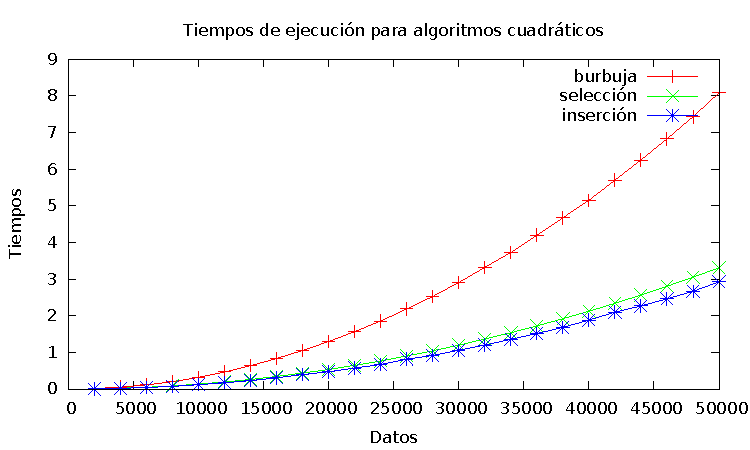
\includegraphics[width=11cm]{comparativa_cuadraticos_g} \centering
	\caption{Algoritmos cuadráticos} \end{figure}

El algoritmo de la burbuja requiere más del doble de tiempo que cualquiera de los otros dos, que se encuentran casi igualados, teniendo un menor tiempo el de inserción. Probablemente este menor tiempo sea el motivo de que en \textit{quicksort} y \textit{mergesort} se use el algoritmo de inserción para subvectores pequeños.

\subsection{Gráfica de los algoritmos $n\cdot log(n)$ }
\begin{figure}[h] 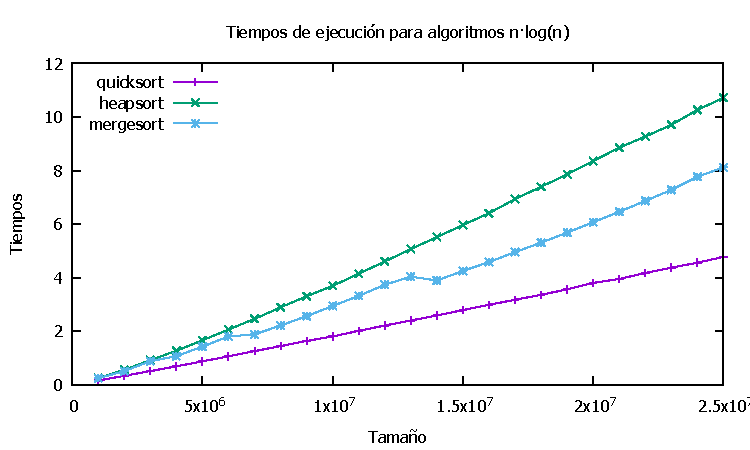
\includegraphics[width=11cm]{comparativa_logaritmicos_g} \centering
	\caption{Algoritmos  $n\cdot log(n)$} \end{figure}

En el algoritmo \textit{mergesort} se aprecian pequeños escalones. Probablemente en cada escalón se incrementa el número de llamadas recursivas, de forma que el tamaño de los subvectores para los que se llama a la función de ordenado por selección (que actúa para tamaños de entrada pequeños) es menor. \\

El algoritmo \textit{quicksort} también usa el algoritmo de inserción por debajo de cierto umbral, pero usa un umbral más pequeño. Esto puede ser la causa de que no presente los escalones.

\newpage
\subsection{Gráfica del algoritmo de Floyd (cúbico)}
\begin{figure}[h] 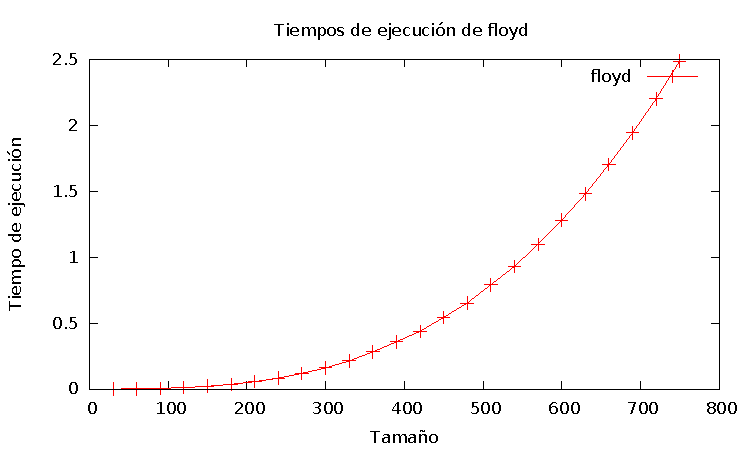
\includegraphics[width=13cm]{floyd_g} \centering
	\caption{Algoritmo de Floyd (cúbico)} \end{figure}

\subsection{Gráfica del algoritmo de Fibonacci $(O(\frac{1+\sqrt{5}}{2})^n)$}
\begin{figure}[h] 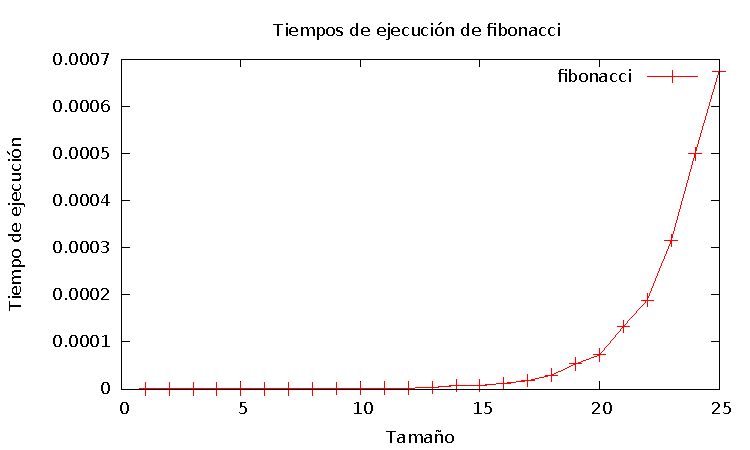
\includegraphics[width=13cm]{fibonacci_g} \centering
	\caption{Algoritmo de Fibonacci} \end{figure}

\newpage
\subsection{Gráfica del algoritmo de Hanoi ($O(2^n)$)}
\begin{figure}[h] 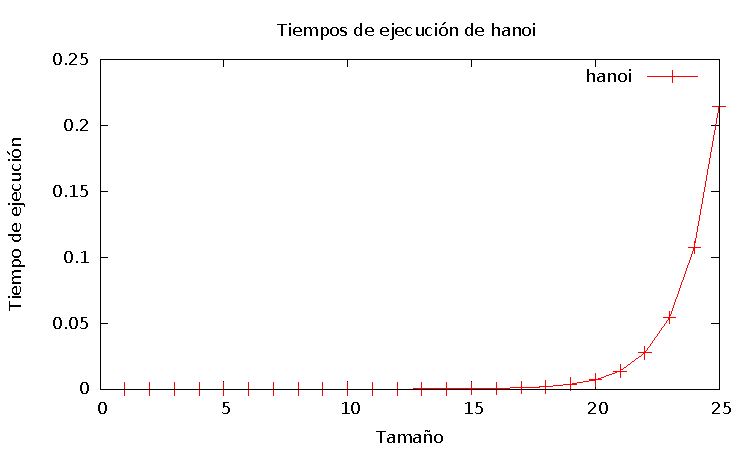
\includegraphics[width=13cm]{hanoi_g} \centering
	\caption{Algoritmo de Hanoi} \end{figure}


\subsection{Gráfica de los algoritmos de ordenación}
\begin{figure}[h] 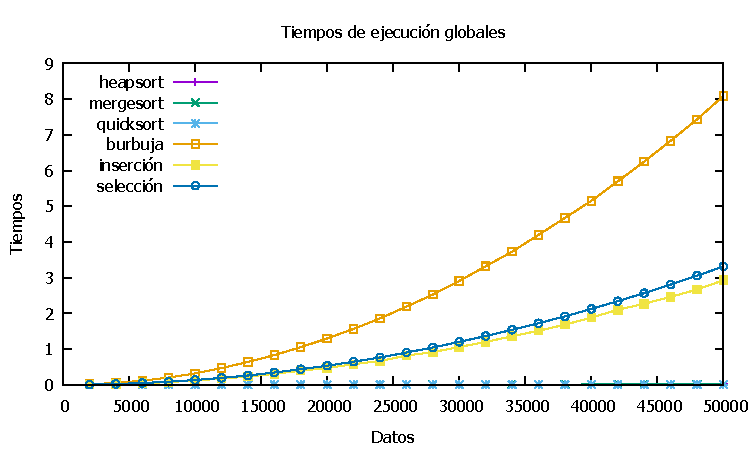
\includegraphics[width=14cm]{comparativa_global_g} \centering
	\caption{Algoritmos de ordenación} \end{figure}

La diferencia en el tiempo de ejecución de los algoritmos de un orden de eficiencia y de otro provoca que los tiempos de los algoritmos de orden de eficiencia $n \cdot \log (n)$ se muestren como una línea horizontal.

\newpage
\section{Ejercicio 3}

\subsection{Eficiencia híbrida de los algoritmos cuadráticos}

\begin{tabular}{|l|l|l|l|}
	\hline
	Persona & Burbuja & Inserción & Selección \\
	\hline
<<<<<<< HEAD
	Pablo & $3\cdot 10^{-9}n^2 -6\cdot 10^{-6}n + 0,015$ & $10^{-9}n^2 + 4\cdot 10^{-7}n + 0,002$ & $10^{-9}n^2 -2\cdot 10^{-7}n + 0,004 (1)$ \\
	Dario &$89\cdot10^{-3} -1.61671\cdot10^{-5}\cdot x +3\cdot10^{-9}\cdot x^2$ &$89 \cdot 10^{-3}+-1.6166\cdot10^{-5} \cdot x +1.68\cdot 10^{-9}\cdot x^2&89\cdot 10^{-3}-1.616\cdot 10^{-5}\cdot x +1.59 \cdot 10^{-9} \cdot x^2 \\
=======
	José Manuel & $3.85\cdot 10^{-9}n^2 - 7.88\cdot 10^{-6}n + 0.013$ ($r=0.999998565269577$) & $1.32\cdot 10^{-9}n^2 + 4.95\cdot 10^{-7}n - 0.0024$ ($r=0.999979582960209$) & $1.59\cdot 10^{-9}n^2 + 2.93 \cdot 10^{-7} n - 0.0022$ $(r=0.999996280002182)$ \\
   \hline
	Pablo & $3\cdot 10^{-9}n^2 -6\cdot 10^{-6}n + 0,015$ ($r=0.99$) & $10^{-9}n^2 + 4\cdot 10^{-7}n + 0,002$ ($r=0.99$) & $10^{-9}n^2 -2\cdot 10^{-7}n + 0,004$ ($r=1$) \\
>>>>>>> master
	\hline
\end{tabular}

\subsection{Eficiencia híbrida de los algoritmos $ n \cdot \log(n)$}

\begin{tabular}{|l|l|l|l|}
	\hline
	Persona & Heapsort & Mergesort & Quicksort \\
	\hline
<<<<<<< HEAD
	Pablo & $1.8 \cdot 10^{-8}n\log(n) -1.9\cdot 10^{-7}$  & $2 \cdot 10^{-8} n \log(n) - 1.9\cdot 10^{-7}$& $1.3 \cdot 10^{-8}n\log(n) -1.9\cdot 10^{-7} (0.999)$\\
=======
   José Manuel & $3.13\cdot 10^{-8}n\log(n) - 0.37$ ($r=0.999702622004366$) & $2.29 \cdot 10^{-8}n\log(n) - 0.082$ ($r=0.997798964368601$) & $1.42 \cdot 10^{-8}n\log(n) + 0.020$ ($r=0.999963309603908$)\\
   \hline
	Pablo & $1.8 \cdot 10^{-8}n\log(n) -1.9\cdot 10^{-7}$ ($r=0.995$)  & $2 \cdot 10^{-8} n \log(n) - 1.9\cdot 10^{-7}$ ($r=0.997$)& $1.3 \cdot 10^{-8}n\log(n) -1.9\cdot 10^{-7}$ ($r=0.999$)\\
>>>>>>> master
	\hline
	Dario &$-0.00499364 +2.58544\cdot 10^{-8}\cdot x\cdot log(x)  $&$ -0.00499364 +3.0260\cdot 10^{-8}\cdot x\cdot log(x)$&$-0.00499364  +1.46227\cdot 10^{-8}\cdot x\cdot log(x) $\\
	\hline
	
\end{tabular}

\subsection{Eficiencia híbrida del algoritmo de Floyd}
\begin{tabular}{|l|l|}
	\hline
	Persona & Eficiencia híbrida de Floyd & Coeficiente de correlación \\
   \hline
 José Manuel & $ 6.88 \cdot 10^{-9}n^3 + 2.89 \cdot 10^{-7}n^2 -4.44 \cdot 10^{-5}n +0.001$ & $0.999960701767451$ \\
	\hline
<<<<<<< HEAD
 Pablo & $ 5.1 \cdot 10^{-9}n^3 + 3.8 \cdot 10^{-7}n^2 -8.3 \cdot 10^{-5}n +0.005$\\
 \hline
 Dario & $ -0.00499364 +0.000217346\cdot x+-7.6610\cdot 10^{-7} + 6.98242\cdot 10^{-9} $ \\
=======
 Pablo & $ 5.1 \cdot 10^{-9}n^3 + 3.8 \cdot 10^{-7}n^2 -8.3 \cdot 10^{-5}n +0.005$ & $1$ \\
>>>>>>> master
 \hline
 
 
\end{tabular}

\subsection{Eficiencia híbrida del algoritmo de Fibonacci}
\begin{tabular}{|l|l|}
	\hline
	Persona & Eficiencia híbrida de Fibonacci & Coeficiente de correlación \\
	\hline
<<<<<<< HEAD
 Pablo & $6.4 \cdot 10^{-9} \frac{1 + \sqrt{5}}{2}^n -1.8\cdot 10^{-8}$\\
=======
 José Manuel & $3.81 \cdot 10^{-9} \frac{1 + \sqrt{5}}{2}^n +9.68\cdot 10^{-7}$ & $0.999939284564366$\\
   \hline
 Pablo & $6.4 \cdot 10^{-9} \frac{1 + \sqrt{5}}{2}^n -1.8\cdot 10^{-8}$ & $0.997$\\
>>>>>>> master
 \hline
 Dario & $-0.00450426 +0.00150218\cdot\phi^x $
\end{tabular}

\subsection{Eficiencia híbrida del algoritmo de Hanoi}
\begin{tabular}{|l|l|}
	\hline
	Persona & Eficiencia híbrida de Hanoi & Coeficiente de correlación \\
	\hline
<<<<<<< HEAD
 Pablo & $6.8 \cdot 10^{-9} 2^n + 1.1 \cdot 10^{-5}$\\
 \hline 
 Dario & $ -0.00499364+ 6.37556\cdot 10^{-9}\cdot 2^x$\\
=======
 José Manuel & $6.00 \cdot 10^{-9} 2^n + 9.3 \cdot 10^{-6}$ & $0.999999531007589$\\
   \hline
 Pablo & $6.1 \cdot 10^{-9} 2^n + 1.1 \cdot 10^{-9}$ & $0.9998$\\
>>>>>>> master
 \hline
\end{tabular}

\end{document}
